\chapter{Tools und Bibliotheken}

In diesem Kapitel werden Bibliotheken und Programme untersucht, die für das Projekt verwendet werden können. 
 
\section{Unterteilungsalgorithmen und Datenstrukturen}

Im Bereich Unterteilungsalgorithmen gibt es viele bereits implementierte Datenstrukturen und Algorithmen.
Gesucht wird eine einfache Datenstruktur, um Polygonnetze verarbeiten zu können.
Diese sollte so wenig Overhead wie möglich mitbringen.
Im Allgemeinen besteht solch eine Datenstruktur aus Ecken (Vertices), Kanten (Edges) und Flächen (Faces).
Zusätzlich muss noch die Beziehung zwischen den Objekten abgespeichert werden.

\subsection{OpenMesh}

OpenMesh wird von der RWTH Aachen entwickelt und stellt eine mächtige Datenstruktur für Polygonnetze bereit.
Es steht unter der LGPL v3 Lizenz (\enquote{with exception}) und kann somit problemlos verwendet werden.

OpenMesh implementiert eine Datenstruktur für Polygonnetze.
Darüber hinaus sind bereits einige Unterteilungsalgorithmen implementiert, die auf der OpenMesh Datenstruktur arbeiten können.
Zum Funktionsumfang gehören folgende Algorithmen:

\begin{enumerate}
\item Uniform subdivision
\begin{itemize}
	\item Loop
	\item Sqrt3
	\item Modified Butterfly
	\item Interpolating Sqrt3
	\item Composite
	\item Catmull Clark
\end{itemize}
\item Adaptive subdivision
\begin{itemize}
	\item Adaptive Composite
\end{itemize}
\item Simple subdivision
\begin{itemize}
	\item Longest Edge
\end{itemize}
\end{enumerate}

OpenMesh implementiert eine \emph{Halfedge} Datenstruktur.
Diese \emph{kantenbasierte} Datenstrukturen speichern die Information über die Verbindungen zwischen Eckpunkten in den Kanten, während
\emph{flächenbasierte} Datenstrukturen die Verbindungsinformation zwischen den Eckpunkten und Nachbarn in den Flächen speichern.

Jede Kante referenziert also folgende Objekte:

\begin{itemize}
	\item zwei Eckpunkte
	\item eine Fläche
	\item die nächsten zwei Kanten der Fläche
\end{itemize}

Halfedge bedeutet nun, dass eine Kante in zwei Halbkanten (Halfedge) aufgeteilt wird. 
Jede Halbkante hat nur eine Richtung.
Zwei Ecken A und B sind also über zwei Halbkanten (erste Halkante von A nach B und zweite Halbkante von B nach A) miteinander verbunden.
Dies bringt den Vorteil, dass man über die Kanten einer Fläche sehr einfach iterieren kann. Man muss dazu lediglich den Halbkanten folgen.


\subsubsection{OpenFlipper}

Aufbauend auf OpenMesh wurde von der RWTH Aachen zusätzlich das flexible Plugin-basierte Framework OpenFlipper enwickelt.
Damit können geometrische Objekte modelliert und verarbeitet werden. Intern wird auf die Datenstrukur OpenMesh zurückgegriffen.
Für die grafische Oberfläche wird QT verwendet.
Mit OpenFlipper kann man über die Oberfläche Netze erstellen und die in OpenMesh implementierten Subdivision Algorithmen anwenden.
\autoref{fig:openflipper} zeigt die Benutzeroberfläche von OpenFlipper.

\begin{figure}
  \centering
  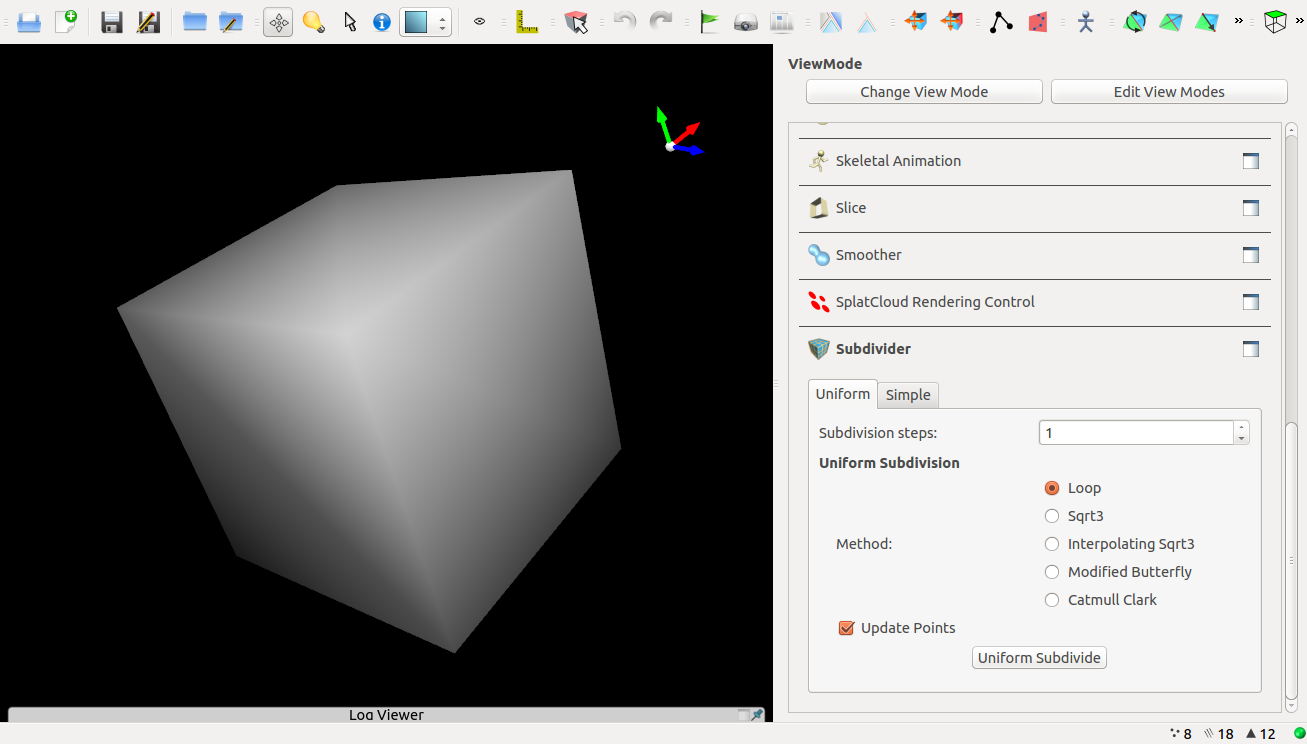
\includegraphics[width=0.8\textwidth]{content/media/openflipper_cube}
  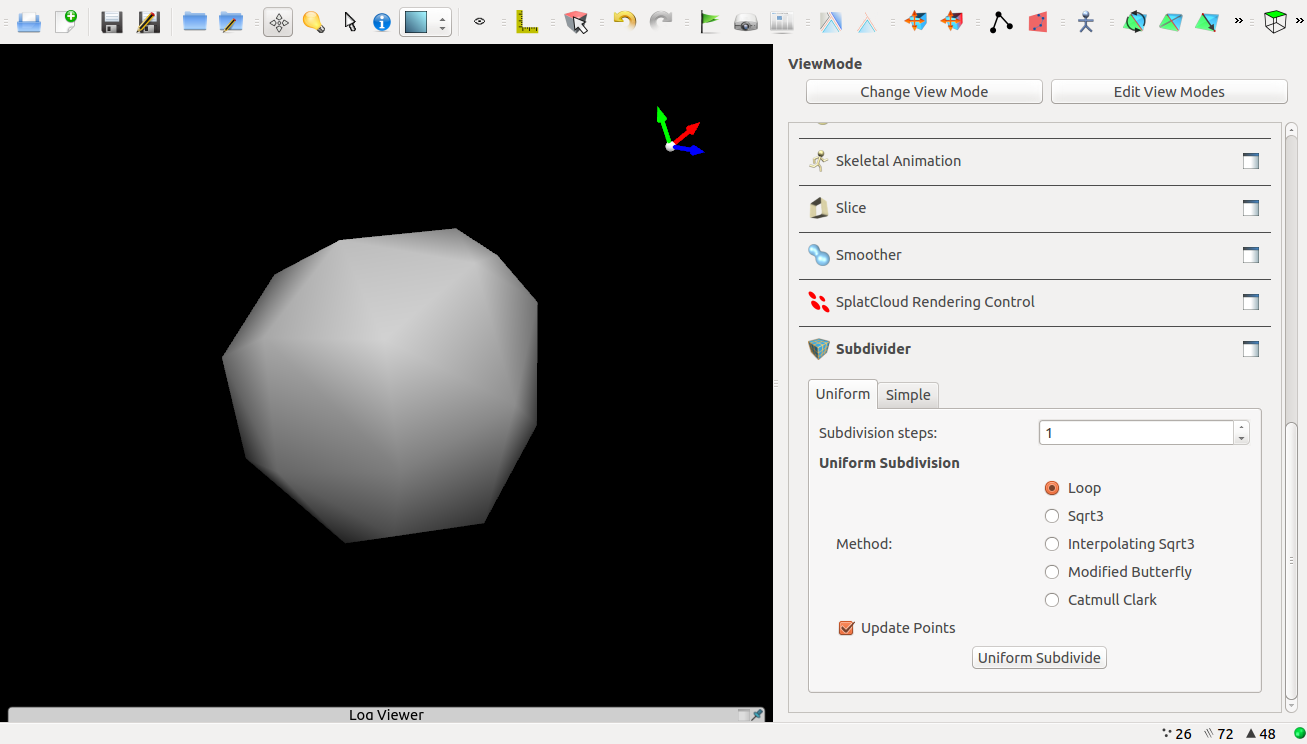
\includegraphics[width=0.8\textwidth]{content/media/openflipper_loop}
  \caption{OpenFlipper}
  \label{fig:openflipper}
\end{figure}


\subsection{Surface\_mesh}

Surface\_mesh \cite{Sieger.} ist eine einfache und effizente Datenstruktur um Polygonnetze beschreiben zu können.
Die Datenstruktur wurde als einfachere Alternative zu OpenMesh von der Bielefeld Graphics \& Geometry Group entwickelt.
Die Datenstruktur soll einfach zu benutzen sein und eine bessere Performance und geringeren Speicherverbrauch mitbringen.
Analog zu OpenMesh implementiert Surface\_mesh eine Halfedge Datenstruktur.
Die Verbindungsinformation der Kanten werden also in einem Paar aus zwei gerichteten Halbkanten gespeichert.
\autoref{fig:sm_halfedge} visualisiert den Zusammenhang der Halbkanten und Ecken.

\begin{figure}
  \centering
  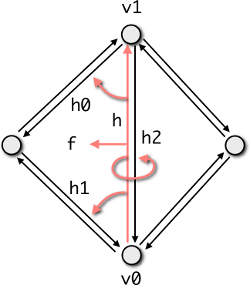
\includegraphics[width=0.3\textwidth]{content/media/sm_connectivity-queries}
  \caption{Surface\_mesh - Halfedge Verbindungen \cite{OpenGP.24.07.2015}}
  \label{fig:sm_halfedge}
\end{figure}

Da Surface\_mesh auch als Halfedge Datenstruktur implementiert ist, kann ähnlich effizient zu OpenMesh über die Kanten iteriert werden.
\autoref{lst:sm_iterate} zeigt einige Basisoperationen die möglich sind.
Die Operationen aus Listing~\ref{lst:sm_iterate} sind zum besseren Verständnis in \autoref{fig:sm_halfedge} gekennzeichnet. 

\begin{lstlisting}[style=myCppStyle, caption=Surface\_mesh - Basisoperationen, label=lst:sm_iterate]
Surface_mesh::Halfedge h;
Surface_mesh::Halfedge h0 = mesh.next_halfedge_handle(h);
Surface_mesh::Halfedge h1 = mesh.prev_halfedge_handle(h);
Surface_mesh::Halfedge h2 = mesh.opposite_halfedge_handle(h);
Surface_mesh::Face     f  = mesh.face_handle(h);
Surface_mesh::Vertex   v0 = mesh.from_vertex_handle(h);
Surface_mesh::Vertex   v1 = mesh.to_vertex_handle(h);
\end{lstlisting}

Um das Netz zu verändern oder zu editieren unterstützt die Datenstruktur high-level Operationen zum Verändern der Topologie.
Mit \emph{Edge Collapse}, \emph{Edge Split} und \emph{Edge Flip} kann das Netz geändert werden.
Die Operationen sind in \autoref{fig:sm_topology} dargestellt. 

\begin{figure}
    \centering
  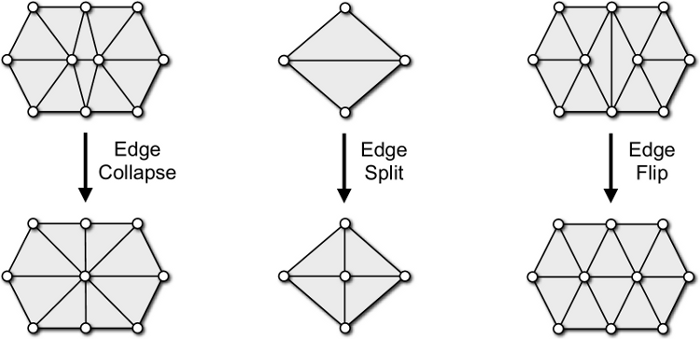
\includegraphics[width=0.8\textwidth]{content/media/sm_topology-changes}
  \caption{Surface\_mesh - high-level Operationen zum Ändern der Topologie \cite{OpenGP.24.07.2015}}
  \label{fig:sm_topology}
\end{figure}

Die Bibliothekt steht unter der \emph{GNU Library General Public License}, was eine problemlose Verwendung in diesem Projekt ermöglicht.

\subsection{OpenSubdiv}

OpenSubdiv wird von Pixar entwickelt und ist eine mächtige Bibliothek, die Unterteilungsalgorithmen und Datenstrukturen implementiert.
Die Bibliothek ist optimiert auf Performance und unterstützt paralleles Rechnen auf CPU und GPU.
Primär wird die Bibliothek von Pixar zum erstellen von animierten Filmen verwendet.
OpenSubdiv ist lizensiert unter der Apache License und darf somit frei für kommerzielle und nicht kommerzielle Projekt genutzt werden.

\begin{figure}
  \centering
  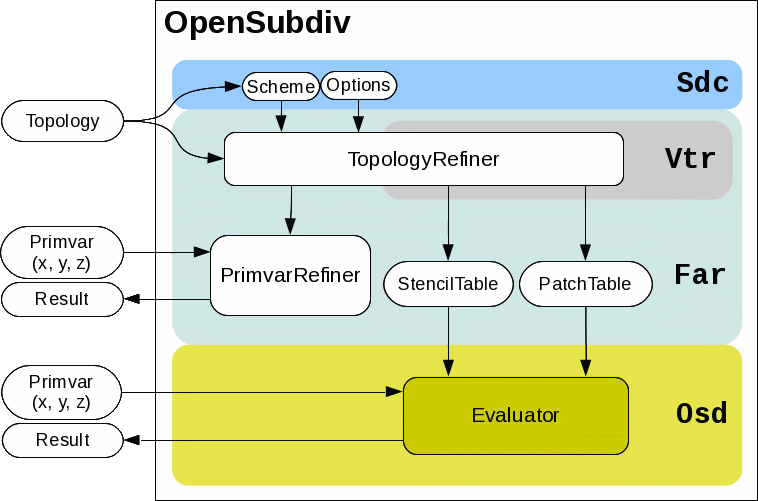
\includegraphics[width=0.9\textwidth]{content/media/pixar_opensubdiv}
  \caption{Pixar OpenSubdiv Architektur \cite{Pixar.27.07.2015}}
  \label{fig:pixar_opensubdiv}
\end{figure}

\autoref{fig:pixar_opensubdiv} zeigt den Aufbau der OpenSubdiv Bibliothek.
Sie besteht insgesamt aus den vier Schichten Sdc, Vtr, Far und Osd \cite{Pixar.27.07.2015}.

\begin{description}
 \item[Sdc] ist die unterste Schicht in der Architektur und implementiert die Unterteilungsdetails.
 Dazu gehören Typen, Optionen und Eigenschaften für die konkreten Unterteilungsalgorithmen.
 \item[Vtr] beinhaltet Klassen, die das Netz für effiziente Verfeinerung in einer Zwischenrepräsentation darstellen.
 Diese Schicht ist nur für den internen Gebrauch gedacht.
 \item[Far] ist die zentrale Schnittstelle, um Polygonnetze mit Unterteilungsalgorithmen zu verarbeiten.
 \item[Osd] beinhaltet geräteabhängigen Code, um Objekte aus der Schicht Far auch in unterschiedlichen Backends wie
  CUDA oder OpenCL ausführbar zu machen.
\end{description}

Von OpenSubdiv werden die Unterteilungsalgorithmen \emph{Catmull-Clark}, \emph{Loop} und \emph{Bilinear} unterstützt \cite{Pixar.27.07.2015}. 

\subsection{CGoGN}

CGoGN ist eine Geometric Modeling C++ Bibliothek und implementiert eine Datenstruktur für n-dimensionale Netze als Combinatorial Maps.
Diese Implementierung unterscheidet sich zu den Halfedge Datenstrukteren von OpenMesh und Surface\_mesh deutlich.
Diese sind zwar alle effizient, haben jedoch Probleme beim Umgang mit Objekten von unterschiedlichen Dimensionen.
Für jeden Problemfall muss die spezielle Datenstruktur verwendet werden.
All diese Strukturen lassen sich jedoch auf Combinatorial Maps zurückführen.
Diesen allgemeineren Ansatz geht CGoGN.
CGoGN implementiert bereits den Unterteilungsalgorithmus Catmull-Clark \cite{CGoGN.27.07.2015}. 

\subsection{Computational Geometry Algorithms Library (CGAL)}

CGAL ist ein mächtiges Softwareprojekt mit einer Vielzahl an Datenstrukturen und Algorithmen.
Neben Unterteilungsalgorithmen werden auch eine Reihe anderer Themengebiete abgedeckt (Voronoi Diagramme, Convex Hull Algorithms, Spatial Searching ...).
Für die Repräsentation von Netzen gibt es bei CGAL mehrere Möglichkeiten.

\begin{description}
 \item[Surface\_mesh] Zum einen implementiert CGAL die bereits vorgestellte Datenstruktur Surface\_mesh.
 \item[3D Polyhedral Surface] Neben Surface\_mesh kann auch die von CGAL entwickelte Halfedge Datenstruktur Polyhedral verwendet werden.
\end{description}

CGAL ist sehr mächtig und komplex. Die Bibliothek ist sogar in den meisten Paketquellen der Linux Distributionen enthalten (z. B. Ubuntu)
und kann darüber sehr leicht installiert werden.
Es sind auch bereits die Unterteilungsalgorithmen \emph{Catmull-Clark}, \emph{Doo-Sabin}, \emph{Loop} und \emph{Sqrt3} implementiert \cite{CGAL.27.07.2015}.

\subsection{Vergleich}

\autoref{tab:sd_bib} gibt einen Überblick über die vorgestellten Bibliotheken und listet auf, welche der ausgewählten Unterteilungsalgorithmen
(Catmull-Clark, Loop, Butterfly und Doo-Sabin) bereits implementiert sind.

\begin{table}
\center
\caption{Vergleich der Unterteilungsalgorithmus Bibliotheken}
\begin{tabular}{l|c|c}
\textbf{Bibliothek} & \textbf{Datenstruktur} & \textbf{Unterteilungsalgorithmen}\\
\hline
\textbf{OpenMesh} & Halfedge & Catmull-Clark, Loop, Butterfly\\
\textbf{Surface\_mesh} & Halfedge & keine\\
\textbf{OpenSubdiv} & Halfedge & Catmull-Clark, Loop\\
\textbf{CGoGN} & combinatorial maps & Catmull-Clark\\
\textbf{CGAL} & Halfedge & Catmull-Clark, Loop, Doo-Sabin\\
\end{tabular}
\label{tab:sd_bib}
\end{table}

Mit Ausnahme von Surface\_mesh, das wirklich nur die Polygonnetz-Datenstruktur mit elementaren Algorithmen implementiert, sind bei den anderen Bibliotheken bereits
einige Unterteilungsalgorithmen implementiert.
Bei Verwendung von OpenMesh oder CGAL könnte man sich viel Arbeit sparen, da dort schon fast alle gewünschten Algorithmen implementiert sind.
Ziel dieses Projektes ist jedoch eine einfache und schnelle Implementierung der Algorithmen.
Surface\_mesh selbst besteht nur aus wenigen Dateien und ist die schlankeste Bibliothek von allen vorgestellten.
\autoref{fig:surface_mesh_cmp} zeigt die Ergebnisse eines Benchmark-Vergleichs für die unterschiedlichen Datenstrukturen.
In dem Diagramm werden die Zeiten relativ zu Surface\_mesh angegeben.

\begin{figure}
  \centering
  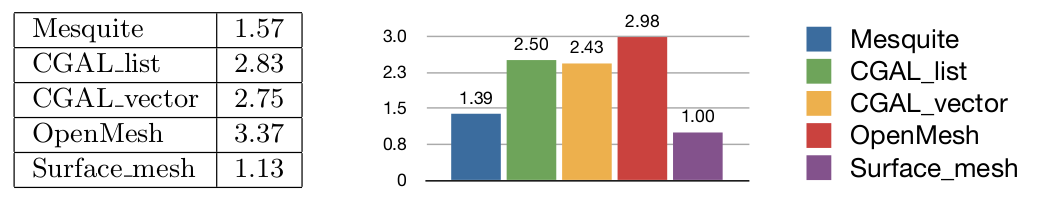
\includegraphics[width=1.0\textwidth]{content/media/surface_mesh_cmp}
   \caption{Benchmarks mit Surface\_mesh \cite{Sieger.}}
  \label{fig:surface_mesh_cmp}
\end{figure}

Man erkennt deutlich, dass die Datenstrukturen von CGAL und OpenMesh vergleichsweise langsam sind.
Da Surface\_mesh sehr kompakt ist (es besteht nur aus sehr wenigen C++ und H-Dateien) und in dem Benchmark auch sehr gute Ergebnisse liefert, fällt die Wahl auf Surface\_mesh.


\section{Rendering}

Im folgenden Unterkapitel werden Bibliotheken und bereits bestehende Software untersucht, mittels derer das Rendering von Polygonnetzen und Limesflächen realisiert werden kann.

Im Gegensatz zur großen Auswahl an unterschiedlichen Möglichkeiten wie beispielsweise bei den Datenstrukturen, beschränkt sich diese hier auf nur wenige Möglichkeiten. Die Wahl ist auf OpenGL wegen seinem großen Funktionsumfang und seiner weiten Verbreitung und auf BezierView auf Grund sehr guter funktionaler Überschneidungen gefallen.


\subsection{OpenGL}

Bei OpenGL handelt es sich um eine sehr weit verbreitete cross-platform Bibliothek für 2-D und 3-D Rendering.
Die API-Spezifikation von OpenGL beinhaltet eine Vielzahl von Befehlen, welche sowohl softwarebasiertes, als auch Hardware beschleunigtes Rendering auf der Grafikkarte ermöglichen. Das ermöglicht eine effiziente Umsetzung des Renderings von Polygonnetzen und Flächen.

Diese Effizienz zeigt sich beispielsweise auch bei Standardoperationen wie dem Draw-Call. Bedingt durch die Verwendung eines internen Zustandsautomaten muss der Befehl lediglich mit den veränderten Parametern aufgerufen werden. OpenGL-Befehle folgen einem konsistenten, sprachunabhängigen Namensschema, welches Informationen zum Aufruf und zur Funktionalität des Befehls enthält. So bezeichnet beispielsweise glVertex3fv() einen OpenGL-Befehl (gl), der einen Eckpunkt definiert (Vertex) und drei (3) float (f) Argumente als Zeiger (v) bekommt.

Ein weiterer Vorteil von OpenGL ist die Lizenzfreiheit für Anwendungsentwickler.


\subsection{BezierView}

BezierView (kurz bview) ist ein einfaches Programm zum Rendern von Bézier Patches, rationalen Bézier Patches und Polygonnetzen 
\\\cite{Peters.bview.27.07.2015}.

Das Programm wurde von Saleh Dindar, Xiaobin Wu, Jorg Peters (University of Florida) entwickelt und ist für Forschungs- und Lehrzwecke als Open Source Projekt frei verfügbar. BezierView ist ebenso wie SubVis in C++ implementiert und verwendet OpenGL für das Rendering.

Überschneidungen ergeben sich besonders beim Rendern der Polygonnetze und der Limesflächen. Die Implementierung von BezierView kann als Grundlage für die konkrete Umsetzung von SubVis verwendet werden.


\section{Grafische Oberfläche}

In diesem Abschnitt werden die Bibliotheken, die für die Darstellung nötig sind, vorgestellt.

\subsection{Qt} % im finalen Bericht (2. Semester) noch ausbauen!

\begin{figure}[hp]
  \centering
  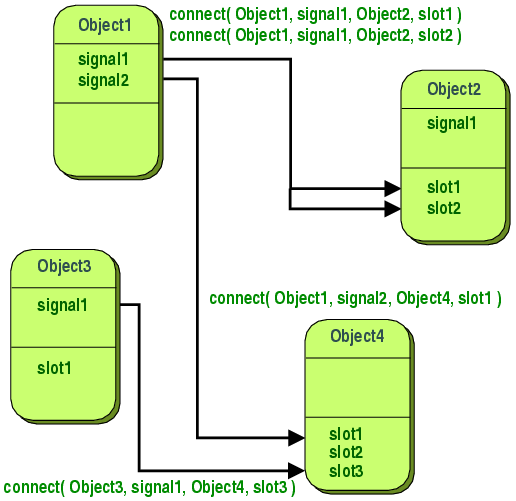
\includegraphics[width=0.6\textwidth]{content/media/qt_signal}
  \caption{Signal-Slots Konzept von Qt \cite{Qt}}
  \label{fig:qt_signal}
\end{figure}

Qt ist eine C++ basierte Bibliothek zur Entwicklung von grafischen Anwendungen \cite{Qt}. 
Der Vorteil von Qt besteht darin, dass die Anwendungen auf den verschiedenen Betriebssystemen annähernd nativ aussehen, in dem wann immer möglich, die nativen Widgets verwendet werden.
Eine Besonderheit von Qt ist das Signals-Slots Konzept (vgl. \autoref{fig:qt_signal}). 
Dieses kann als eine Art Beobachter-Entwurfsmuster betrachtet werden.
Dabei entspricht ein Signal einem \emph{notify} und ein Slot einem \emph{Beobachter}. 
Mittels einer \emph{connect} Funktion wird die Verbindung zwischen den Komponenten (n:m) hergestellt.
Zur Definition von Signalen und Slots werden Makros verwendet, die vom Meta-Object-Compiler \emph{moc} in standardkonformen C++ Code umgewandelt werden.
Qt wird unter der LGPL verteilt.

\subsection{libQGLViewer} % im finalen Bericht (2. Semester) noch ausbauen!

Die Bibliothek bietet einige grundlegende Funktionen zur Erstellung von 3D OpenGL Betrachtern mit C++ \cite{libQGLViewer}.
Sie bietet unter anderem folgende Funktionen bzw. erleichtert deren Erstellung:

\begin{itemize}
\item Mit der Maus verschiebbare Kamera
\item Weltkoordinatensystem
\item Verschiebung von Koordinatensystem und Objekten
\item Frame-Animation
\item Objektselektion mit der Maus
\item Screenshots
\item Tastaturkürzel und Maus-Bindings
\end{itemize}

Die Software ist unter der GPL frei verfügbar.

\section{IDE} % im finalen Bericht (2. Semester) noch ausbauen!

In Bezug auf Qt und C++ bietet sich die IDE \emph{Qt Creator} \cite{QtCreator} an. 
Diese bietet alle gewohnten Funktionen einer IDE wie Syntaxhervorhebung, Autovervollständigung, GUI-Designer, Debugger und Git-Integration.
Insbesondere der GUI-Designer nimmt viel Arbeit ab, da so einiges an Boilerplate-Code automatisch erzeugt werden kann.

Projekte werden in sog. \emph{.pro} Dateien konfiguriert. 
Diese Datei ist plattformunabhängig und relativ schlank gehalten. 
Erst bei Ausführung durch qmake wird ein plattformspezifisches Makefile generiert, welches dann mittels Make ausgeführt werden kann.

\section{Dokumentation} % im finalen Bericht (2. Semester) noch ausbauen!

Im Bereich C++ ist Doxygen \cite{Doxygen} eine weit verbreitete Quellcodedokumentationslösung.
Prinzipiell ähnelt es JavaDoc, in dem Quellcode direkt mittels spezielle annotierten Kommentaren versehen wird.
Diese Annotationen werden dann mittels Transformation in ein Ausgabeformat (z. B. HTML oder PDF) überführt.
Der Vorteil liegt darin, dass so die Dokumentation sehr nahe und eng mit dem Quellcode verbunden ist, was die Aktualität der Dokumentation begünstigt.
Qt Creator bietet Syntaxhervorhebung für die speziellen Kommentare und erleichtert so die Verwendung.
Doxygen steht unter der GPL.
